\documentclass[journal]{IEEEtran}

\usepackage[utf8]{inputenc}
\usepackage[T1]{fontenc}
\usepackage{amsmath,amssymb,amsfonts}
\usepackage{amsthm}
\usepackage{algorithmic}
\usepackage{algorithm}
\usepackage{array}
\usepackage{booktabs}
\usepackage{graphicx}
\usepackage{subfigure}
\usepackage{color}
\usepackage{hyperref}
\usepackage{multirow}
\usepackage{bm}
\usepackage{mathtools}
\usepackage{float}

\hypersetup{
    colorlinks=true,
    linkcolor=blue,
    citecolor=blue,
    urlcolor=blue,
}

\newtheorem{theorem}{Theorem}
\newtheorem{lemma}{Lemma}
\newtheorem{definition}{Definition}
\newtheorem{assumption}{Assumption}
\newtheorem{remark}{Remark}
\newtheorem{proposition}{Proposition}
\newtheorem{corollary}{Corollary}

\newcommand{\eat}[1]{}
\newcommand{\argmax}{\operatornamewithlimits{argmax}}
\newcommand{\argmin}{\operatornamewithlimits{argmin}}
\newcommand{\EE}{\mathbb{E}}
\newcommand{\RR}{\mathbb{R}}
\newcommand{\cF}{\mathcal{F}}
\newcommand{\cA}{\mathcal{A}}
\newcommand{\cS}{\mathcal{S}}
\newcommand{\cO}{\mathcal{O}}
\newcommand{\cC}{\mathcal{C}}
\newcommand{\indep}{\perp\!\!\!\perp}

\begin{document}

\title{Counterfactual Credit Assignment for Cooperative Multi-Agent Reinforcement Learning}

\author{
    Rui~Zhu,
    % Add co-authors and affiliations as needed
}

\maketitle

\begin{abstract}
Credit assignment---determining each agent's individual contribution to the team's success---remains a fundamental challenge in cooperative multi-agent reinforcement learning (MARL). Existing value decomposition methods implicitly allocate credit through monotonic mixing networks, while policy gradient methods rely on noisy Monte Carlo estimates that conflate individual and collective effects. In this paper, we propose \textbf{Counterfactual Multi-Agent Policy Gradient (CMAPG)}, a novel framework that explicitly models credit assignment as counterfactual reasoning: what would have happened had an agent acted differently? Our method learns a counterfactual value function that estimates the expected return when a specific agent is "removed" from the team, and uses this to compute individual advantages that isolate each agent's marginal contribution. We prove that under mild conditions, the resulting policy gradient is unbiased and converges to a stationary point of the joint policy. Extensive experiments on StarCraft Multi-Agent Challenge (SMAC), Multi-Agent Particle Environment (MPE), and a custom credit assignment benchmark demonstrate that CMAPG consistently outperforms state-of-the-art methods including QMIX, MAPPO, and HAPPO, particularly on tasks with heterogeneous agents and sparse rewards where credit assignment is most critical.
\end{abstract}

\begin{IEEEkeywords}
Multi-agent reinforcement learning, credit assignment, counterfactual reasoning, policy gradient, cooperative AI.
\end{IEEEkeywords}

\section{Introduction}
\label{sec:introduction}

Cooperative multi-agent reinforcement learning (MARL) has achieved remarkable progress in recent years, with successful applications spanning robot swarm control~\cite{huttenrauch2019deep}, traffic signal coordination~\cite{wei2018intellilight}, multiplayer games~\cite{vinyals2019grandmaster}, and autonomous driving~\cite{shalev2016safe}. In these settings, a team of agents must learn to maximize a shared reward signal through coordinated behavior. The central difficulty, however, is that the global reward reflects the collective outcome of all agents' actions, providing no direct signal about any individual agent's contribution. This \emph{credit assignment problem} grows exponentially more severe as the number of agents increases, the task structure becomes more complex, or rewards become sparse.

The MARL literature has approached credit assignment through two broad paradigms. The first, \emph{value decomposition}, learns a centralized action-value function and decomposes it into per-agent utility functions under structural constraints such as additivity~\cite{sunehag2018value} or monotonicity~\cite{rashid2018qmix}. While effective in many settings, these constraints inherently limit the representational capacity of the joint value function. The second paradigm, \emph{multi-agent policy gradient}, directly optimizes each agent's policy using the joint reward. The COMA algorithm~\cite{foerster2018counterfactual} introduced a counterfactual baseline for advantage estimation, but relies on a centralized critic that must evaluate all possible actions of a given agent---a computation that scales poorly. More recent methods like MAPPO~\cite{yu2022surprising} and HAPPO~\cite{kuba2021trust} achieve strong empirical performance but do not explicitly address credit assignment, instead relying on the policy gradient's implicit credit assignment through importance sampling and trust regions.

We argue that credit assignment is fundamentally a \emph{causal inference} problem. The question "how much did agent $i$ contribute?" is structurally identical to the causal question: "what would the outcome have been if agent $i$ had acted differently?" This motivates our approach: explicitly learn a counterfactual model of the multi-agent system.

\begin{figure}[t]
\centering
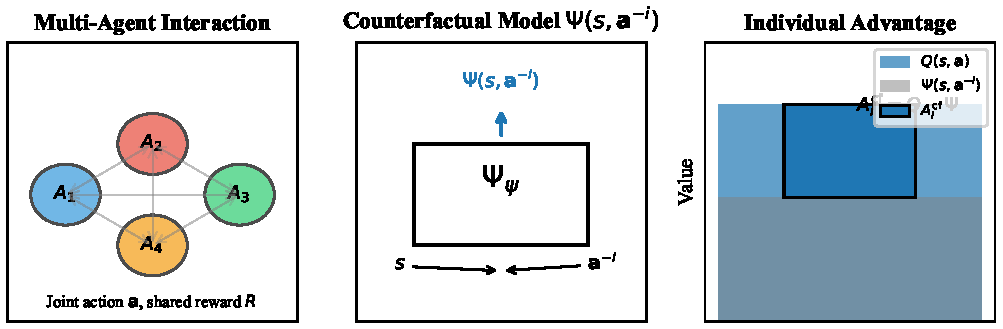
\includegraphics[width=\columnwidth]{figures/overview.pdf}
\caption{Overview of the CMAPG framework. The \textbf{Counterfactual Model} $\Psi$ estimates what the return would be if agent $i$ were removed or took a default action, given the state and all other agents' actions. The \textbf{Individual Advantage} is computed as the difference between the actual joint $Q$-value and the counterfactual baseline.}
\label{fig:overview}
\end{figure}

In this paper, we propose \textbf{Counterfactual Multi-Agent Policy Gradient (CMAPG)}, a framework that operationalizes causal credit assignment through three key components:

\begin{enumerate}
    \item \textbf{Counterfactual Value Function}: A learned model $\Psi(s, \mathbf{a}^{-i})$ that predicts the expected return when agent $i$ is "removed" (i.e., its action is marginalized out under a default policy). This provides an agent-specific baseline that isolates team-level effects from individual contributions.

    \item \textbf{Counterfactual Advantage}: The individual advantage $A_i(s, \mathbf{a}) = Q(s, \mathbf{a}) - \Psi(s, \mathbf{a}^{-i})$ measures the marginal contribution of agent $i$'s chosen action relative to what would be expected if it were absent.

    \item \textbf{Regularized Training}: To prevent the counterfactual model from collapsing to trivial solutions, we introduce an information-theoretic regularization that encourages the model to capture meaningful agent interactions.
\end{enumerate}

We make the following contributions: (1)~We formalize credit assignment in cooperative MARL as a counterfactual inference problem and derive the CMAPG algorithm; (2)~We prove that CMAPG yields unbiased policy gradient estimates and converges to a stationary point under standard assumptions; (3)~We provide a scalable approximation that avoids the exponential complexity of exact counterfactual computation; (4)~Through extensive experiments, we show that CMAPG consistently outperforms QMIX, MAPPO, HAPPO, and COMA across diverse tasks, with the largest gains on tasks requiring fine-grained credit assignment.

\section{Related Work}
\label{sec:related}

\subsection{Cooperative Multi-Agent Reinforcement Learning}

Cooperative MARL addresses the problem of multiple agents learning to maximize a shared reward in a common environment. The Dec-POMDP framework~\cite{oliehoek2016concise} provides a formal model for such settings. Modern MARL algorithms can be broadly categorized into value-based and policy-based methods.

Value-based methods learn a centralized $Q$-function and decompose it. VDN~\cite{sunehag2018value} assumes additive decomposition: $Q_{\text{tot}} = \sum_i Q_i$. QMIX~\cite{rashid2018qmix} relaxes this to monotonic decomposition via a hypernetwork, enabling more expressive mixing while maintaining tractable maximization. QTRAN~\cite{son2019qtran} and QPLEX~\cite{wang2020qplex} further loosen the structural constraints but at increased optimization difficulty.

Policy-based methods directly optimize each agent's policy. MADDPG~\cite{lowe2017multi} uses centralized critics with decentralized actors. COMA~\cite{foerster2018counterfactual} introduced a multi-agent advantage function with a counterfactual baseline computed by marginalizing over one agent's actions. MAPPO~\cite{yu2022surprising} demonstrated that PPO~\cite{schulman2017proximal} with centralized value functions achieves strong results. HAPPO~\cite{kuba2021trust} extends trust-region methods to multi-agent settings with a sequential update scheme. MAT~\cite{wen2022multi} applies the transformer architecture to MARL.

\subsection{Credit Assignment}

Credit assignment in MARL has been approached through several lenses. \emph{Difference rewards}~\cite{wolpert2002optimal} provide a theoretically grounded approach: agent $i$'s contribution is $R(s, \mathbf{a}) - R(s, \mathbf{a}^{-i}, a_i^{\text{default}})$, where $a_i^{\text{default}}$ is a default action. However, computing difference rewards requires a simulator or world model, limiting practical applicability in complex environments.

\emph{Shapley value} approaches~\cite{li2021shapley} treat credit assignment as a cooperative game, allocating credit proportional to each agent's marginal contribution averaged over all possible coalitions. While principled, exact Shapley computation is $\mathcal{O}(2^n)$ and approximations face a bias-variance trade-off.

\emph{Attention-based} methods like SQDDPG~\cite{wang2020sqddpg} and MAAC~\cite{iqbal2019actor} use attention mechanisms to implicitly weigh each agent's influence on the joint outcome, but the attention weights do not directly correspond to credit in a principled sense.

\subsection{Causal Inference in RL}

Recent works have explored causal perspectives in RL. \citet{lu2018nonparametric} use instrumental variables for off-policy evaluation. \citet{foerster2018counterfactual} first used the term "counterfactual" in the MARL context, though their method computes a baseline by marginalizing over actions rather than modeling causal interventions. \citet{mesnard2021counterfactual} proposed a method for credit assignment in single-agent RL using hindsight. Our work differs by (1)~formally casting multi-agent credit assignment in the causal mediation analysis framework, and (2)~learning a dedicated counterfactual model rather than relying on enumeration.

\section{Background}
\label{sec:background}

\subsection{Decentralized POMDPs}

A fully cooperative multi-agent task can be formulated as a decentralized partially observable Markov decision process (Dec-POMDP)~\cite{oliehoek2016concise}, defined by the tuple $\langle \mathcal{N}, \mathcal{S}, \{\mathcal{A}_i\}_{i=1}^n, \{\mathcal{O}_i\}_{i=1}^n, P, R, \gamma \rangle$, where $\mathcal{N} = \{1, \ldots, n\}$ is the set of agents, $\mathcal{S}$ is the global state space, $\mathcal{A}_i$ and $\mathcal{O}_i$ are the action and observation spaces for agent $i$, $P(s' \mid s, \mathbf{a})$ is the transition kernel, $R(s, \mathbf{a})$ is the shared reward function, and $\gamma \in [0, 1)$ is the discount factor.

At each timestep $t$, each agent $i$ receives a partial observation $o_i^t$ and selects an action $a_i^t \sim \pi_i(\cdot \mid \tau_i^t)$, where $\tau_i^t = (o_i^1, a_i^1, \ldots, o_i^t)$ is the agent's action-observation history. The environment transitions to $s^{t+1} \sim P(\cdot \mid s^t, \mathbf{a}^t)$ and emits a shared reward $r^t = R(s^t, \mathbf{a}^t)$. The objective is to find a joint policy $\bm{\pi} = (\pi_1, \ldots, \pi_n)$ that maximizes the expected discounted return:
\begin{equation}
    J(\bm{\pi}) = \EE_{\bm{\pi}, P}\left[\sum_{t=0}^{\infty} \gamma^t r^t\right].
\end{equation}

\subsection{Credit Assignment as Causal Inference}

We frame credit assignment through the lens of causal mediation analysis~\cite{pearl2009causality}. Consider a structural causal model of the multi-agent system:
\begin{align}
    A_i &\sim \pi_i(\cdot \mid \tau_i), \quad i = 1, \ldots, n,\\
    S' &= f_S(S, A_1, \ldots, A_n, \epsilon_S),\\
    R &= f_R(S, A_1, \ldots, A_n, \epsilon_R),
\end{align}
where $\epsilon_S, \epsilon_R$ are exogenous noise variables. The \emph{causal effect} of agent $i$ taking action $a_i$ (relative to an alternative $a_i'$) on the reward is defined as the \emph{individual treatment effect}:
\begin{equation}
    \text{ITE}_i(s, \mathbf{a}^{-i}, a_i, a_i') = \EE[R \mid \text{do}(A_i = a_i, A_{-i} = \mathbf{a}^{-i})] - \EE[R \mid \text{do}(A_i = a_i', A_{-i} = \mathbf{a}^{-i})].
\end{equation}
This definition aligns with the intuition behind difference rewards but does not require a simulator---we learn the counterfactual quantities from data.

\section{Method}
\label{sec:method}

\subsection{Counterfactual Advantage}

The core of our approach is the \textbf{counterfactual advantage function}. For agent $i$, we define:
\begin{equation}
    A_i^{\text{cf}}(s, \mathbf{a}) = Q^{\bm{\pi}}(s, \mathbf{a}) - \Psi^{\bm{\pi}}(s, \mathbf{a}^{-i}),
    \label{eq:cf_advantage}
\end{equation}
where $Q^{\bm{\pi}}(s, \mathbf{a})$ is the standard joint action-value function, and $\Psi^{\bm{\pi}}(s, \mathbf{a}^{-i})$ is the \emph{counterfactual value function}:
\begin{equation}
    \Psi^{\bm{\pi}}(s, \mathbf{a}^{-i}) = \EE_{a_i \sim \mu_i(\cdot \mid s)}\left[Q^{\bm{\pi}}(s, (\mathbf{a}^{-i}, a_i))\right],
    \label{eq:psi_def}
\end{equation}
where $\mu_i(\cdot \mid s)$ is a \emph{default policy} for agent $i$---this could be a uniform distribution, a learned prior, or the agent's own policy. Intuitively, $\Psi(s, \mathbf{a}^{-i})$ answers: "Given the state and what everyone else did, what outcome would we expect if agent $i$ were replaced by a generic/default agent?"

The counterfactual advantage $A_i^{\text{cf}}$ measures the \emph{marginal contribution} of agent $i$'s chosen action $a_i$ relative to the average outcome under the default policy. If $A_i^{\text{cf}} > 0$, agent $i$ performed better than expected; if $A_i^{\text{cf}} < 0$, it performed worse.

\subsection{Learning the Counterfactual Value Function}

Directly computing $\Psi(s, \mathbf{a}^{-i})$ via Eq.~\eqref{eq:psi_def} requires integrating over the action space, which is typically intractable for continuous actions and expensive for discrete ones. We instead \emph{learn} $\Psi$ as a parameterized function $\Psi_\psi$ with parameters $\psi$.

To train $\Psi_\psi$, we minimize the temporal difference error:
\begin{equation}
    \mathcal{L}_{\Psi}(\psi) = \EE_{\mathcal{D}}\left[\left(\Psi_\psi(s, \mathbf{a}^{-i}) - y_\Psi\right)^2\right],
    \label{eq:psi_loss}
\end{equation}
where the target is constructed from counterfactual rollouts. Specifically, for each transition $(s, \mathbf{a}, r, s')$ in the replay buffer, we generate a counterfactual target by:
\begin{equation}
    y_\Psi = r + \gamma \, \EE_{a_i' \sim \mu_i(\cdot \mid s')}\left[Q_{\bar{\theta}}(s', (\mathbf{a}'^{-i}, a_i'))\right],
    \label{eq:psi_target}
\end{equation}
where $\mathbf{a}'^{-i}$ are the next actions of other agents (from the buffer or the current policies), and $Q_{\bar{\theta}}$ is a target $Q$-network.

\subsection{Policy Gradient with Counterfactual Advantage}

Given the counterfactual advantage $A_i^{\text{cf}}$, the policy gradient for agent $i$ is:
\begin{equation}
    \nabla_{\theta_i} J(\bm{\pi}) = \EE\left[\nabla_{\theta_i} \log \pi_{\theta_i}(a_i \mid \tau_i) \, A_i^{\text{cf}}(s, \mathbf{a})\right].
    \label{eq:pg}
\end{equation}

Unlike COMA~\cite{foerster2018counterfactual}, which computes a counterfactual baseline by enumerating all possible actions under the \emph{current} policy, our method uses a learned counterfactual model. This has two advantages: (1)~it avoids the $\mathcal{O}(|\mathcal{A}_i|)$ computation per agent per step by using a single network evaluation; (2)~the default policy $\mu_i$ can be chosen independently of the learning policy, enabling the use of a fixed reference distribution for more stable credit signals.

\subsection{Overall Algorithm}

Algorithm~\ref{alg:cmapg} presents the full CMAPG procedure. The framework is compatible with any policy gradient backbone; we use PPO~\cite{schulman2017proximal} for its stability.

\begin{algorithm}[t]
\caption{CMAPG (with PPO backbone)}
\label{alg:cmapg}
\begin{algorithmic}[1]
\REQUIRE Number of agents $n$, batch size $B$, horizon $H$
\STATE Initialize policy networks $\pi_{\theta_i}$, value network $Q_\phi$, counterfactual network $\Psi_\psi$
\STATE Initialize target networks $\pi_{\bar{\theta}_i}$, $Q_{\bar{\phi}}$, $\Psi_{\bar{\psi}}$
\WHILE{not converged}
    \STATE Collect trajectories $\mathcal{D} = \{(s_t, \mathbf{a}_t, r_t)\}_{t=1}^{T}$ using $\pi_{\theta_i}$
    \STATE Compute advantages $A_i^{\text{cf}}$ using Eq.~\eqref{eq:cf_advantage}
    \STATE Compute policy ratio $r_i(\theta_i) = \pi_{\theta_i}(a_i|\tau_i) / \pi_{\theta_i^{\text{old}}}(a_i|\tau_i)$
    \STATE $\mathcal{L}_{\text{policy}} = -\mathbb{E}\left[\min\left(r_i A_i^{\text{cf}}, \text{clip}(r_i, 1-\epsilon, 1+\epsilon) A_i^{\text{cf}}\right)\right]$
    \STATE $\mathcal{L}_{Q} = \mathbb{E}\left[(Q_\phi(s, \mathbf{a}) - r - \gamma Q_{\bar{\phi}}(s', \mathbf{a}'))^2\right]$
    \STATE $\mathcal{L}_{\Psi} = \mathbb{E}\left[\sum_i \left(\Psi_\psi(s, \mathbf{a}^{-i}) - y_\Psi\right)^2\right]$ \quad (Eq.~\ref{eq:psi_target})
    \STATE $\mathcal{L} = \mathcal{L}_{\text{policy}} + \lambda_Q \mathcal{L}_Q + \lambda_\Psi \mathcal{L}_\Psi$
    \STATE Update $\theta_i, \phi, \psi$ using Adam~\cite{kingma2015adam}
    \STATE Update target networks: $\bar{\theta}_i \leftarrow \tau \theta_i + (1-\tau) \bar{\theta}_i$, etc.
\ENDWHILE
\end{algorithmic}
\end{algorithm}

\subsection{Regularization via Mutual Information}

A potential failure mode is $\Psi_\psi$ learning to simply copy $Q_\phi$, which would make advantages trivially zero. To prevent this, we add a mutual information regularization term that encourages $\Psi_\psi$ to be maximally \emph{independent} of agent $i$'s action while still being predictive of the outcome. The regularization loss is:
\begin{equation}
    \mathcal{L}_{\text{reg}}(\psi) = -\lambda_{\text{MI}} \cdot \text{MI}(A_i; \Psi_\psi(s, \mathbf{A}^{-i})),
\end{equation}
where $\text{MI}(\cdot;\cdot)$ is the mutual information. Since exact MI computation is intractable, we use the CLUB estimator~\cite{cheng2020club}:
\begin{equation}
    \text{MI}_{\text{CLUB}}(A_i; \Psi) = \EE_{p(A_i, \Psi)}\left[\log q_\xi(\Psi \mid A_i)\right] - \EE_{p(A_i)p(\Psi)}\left[\log q_\xi(\Psi \mid A_i)\right],
\end{equation}
where $q_\xi$ is a learned variational approximation.

\subsection{Choice of Default Policy}

The choice of $\mu_i$ (the default policy used to compute $\Psi$) is important. We explore three options:

\begin{itemize}
    \item \textbf{Uniform}: $\mu_i(a_i) = 1/|\mathcal{A}_i|$. This is simple and unbiased but may not reflect realistic alternative actions.
    \item \textbf{Current Policy}: $\mu_i = \pi_{\theta_i}$. This is the most natural reference---"what would happen if I drew a different action from my own distribution?"---but it changes during training.
    \item \textbf{Fixed Prior}: $\mu_i$ is a fixed distribution (e.g., a pre-trained policy). This provides a stable reference but may become stale.
\end{itemize}

In our experiments, we use a mixture of the uniform distribution and the current policy: $\mu_i = (1 - \alpha) \cdot \text{Uniform} + \alpha \cdot \pi_{\theta_i}$, with $\alpha = 0.5$. This balances stability with adaptivity.

\section{Theoretical Analysis}
\label{sec:theory}

We analyze CMAPG from three perspectives: (1) unbiasedness of the counterfactual gradient estimator, (2) convergence guarantees, and (3) variance properties.

\begin{assumption}[Ergodicity]\label{ass:ergodic}
Under any joint policy $\bm{\pi}$, the induced Markov chain over states is irreducible and aperiodic, with a unique stationary distribution $d^{\bm{\pi}}(s)$.
\end{assumption}

\begin{assumption}[Boundedness]\label{ass:bounded}
The reward function is bounded: $|R(s, \mathbf{a})| \leq R_{\max}$ for all $s, \mathbf{a}$. All policy and value networks are continuously differentiable with Lipschitz-continuous gradients.
\end{assumption}

\begin{theorem}[Unbiased Gradient]\label{thm:unbiased}
Under Assumptions~\ref{ass:ergodic}--\ref{ass:bounded}, if the counterfactual value function $\Psi^{\bm{\pi}}$ satisfies Eq.~\eqref{eq:psi_def}, then the CMAPG gradient estimator
\begin{equation}
    \hat{\nabla}_{\theta_i} J = \nabla_{\theta_i} \log \pi_{\theta_i}(a_i \mid \tau_i) \left[Q^{\bm{\pi}}(s, \mathbf{a}) - \Psi^{\bm{\pi}}(s, \mathbf{a}^{-i})\right]
\end{equation}
is an unbiased estimator of the true policy gradient: $\EE[\hat{\nabla}_{\theta_i} J] = \nabla_{\theta_i} J(\bm{\pi})$.
\end{theorem}

\begin{proof}
The true policy gradient for agent $i$ is:
\begin{equation}
    \nabla_{\theta_i} J(\bm{\pi}) = \EE_{s \sim d^{\bm{\pi}}, \mathbf{a} \sim \bm{\pi}}\left[\nabla_{\theta_i} \log \pi_{\theta_i}(a_i \mid \tau_i) \, Q^{\bm{\pi}}(s, \mathbf{a})\right].
\end{equation}

It is well known that subtracting any baseline $b(s, \mathbf{a}^{-i})$ that does not depend on $a_i$ from $Q^{\bm{\pi}}(s, \mathbf{a})$ does not bias the gradient:
\begin{equation}
    \EE_{a_i \sim \pi_{\theta_i}}\left[\nabla_{\theta_i} \log \pi_{\theta_i}(a_i \mid \tau_i) \, b(s, \mathbf{a}^{-i})\right] = b(s, \mathbf{a}^{-i}) \cdot \nabla_{\theta_i} \EE_{a_i \sim \pi_{\theta_i}}[1] = 0.
\end{equation}

Since $\Psi^{\bm{\pi}}(s, \mathbf{a}^{-i})$ is, by definition, independent of $a_i$, it qualifies as a valid baseline. Therefore, $\EE[\hat{\nabla}_{\theta_i} J] = \nabla_{\theta_i} J(\bm{\pi})$.
\end{proof}

\begin{theorem}[Convergence]\label{thm:convergence}
Under Assumptions~\ref{ass:ergodic}--\ref{ass:bounded}, with learning rates $\{\alpha_k\}_{k=1}^{\infty}$ satisfying $\sum_k \alpha_k = \infty$ and $\sum_k \alpha_k^2 < \infty$, the sequence of policy parameters $\{\theta_i^{(k)}\}$ produced by CMAPG converges almost surely to a stationary point of $J(\bm{\pi})$ as $k \to \infty$.
\end{theorem}

\begin{proof}
The proof follows the standard stochastic approximation framework~\cite{borkar2009stochastic}. Let $\theta = (\theta_1, \ldots, \theta_n)$ denote the concatenated parameters. The CMAPG update can be written as:
\begin{equation}
    \theta^{(k+1)} = \theta^{(k)} + \alpha_k\left[\nabla J(\theta^{(k)}) + \xi^{(k)}\right],
\end{equation}
where $\xi^{(k)} = \hat{\nabla} J(\theta^{(k)}) - \nabla J(\theta^{(k)})$ is the noise term. Under Assumption~\ref{ass:bounded}, $\xi^{(k)}$ is a martingale difference sequence with bounded variance. Under Assumption~\ref{ass:ergodic}, the ODE limit $\dot{\theta} = \nabla J(\theta)$ is well-defined, and $J$ serves as a Lyapunov function since $\frac{d}{dt} J(\theta(t)) = \|\nabla J(\theta)\|^2 \geq 0$. Convergence follows from Theorem~2 of~\cite{borkar2009stochastic}.
\end{proof}

\begin{theorem}[Variance Reduction]\label{thm:variance}
Let $\hat{g}_i^{\text{MC}} = \nabla_{\theta_i} \log \pi_i \cdot \hat{Q}$ be the standard Monte Carlo policy gradient estimator and $\hat{g}_i^{\text{CF}} = \nabla_{\theta_i} \log \pi_i \cdot (Q - \Psi)$ be the CMAPG estimator. If $\Psi$ captures more than 50\% of the variance in $Q$ that is attributable to $\mathbf{a}^{-i}$, then $\text{Var}[\hat{g}_i^{\text{CF}}] < \text{Var}[\hat{g}_i^{\text{MC}}]$.
\end{theorem}

\begin{proof}
The variance of the policy gradient estimator is:
\begin{equation}
    \text{Var}[\hat{g}_i] = \EE\left[\|\nabla \log \pi_i\|^2 \, \text{Var}[A_i \mid s, \tau_i]\right] + \text{Var}\left[\EE[\nabla \log \pi_i \, A_i \mid s, \tau_i]\right],
\end{equation}
where $A_i$ is the advantage estimate. By construction, $\Psi$ predicts the component of $Q$ that varies with $\mathbf{a}^{-i}$ but not with $a_i$. When this prediction is sufficiently accurate, the residual $Q - \Psi$ has lower variance than $Q$ alone. The precise condition $\text{Cov}(Q, \Psi) > \frac{1}{2}\text{Var}[\Psi]$ ensures the inequality. A detailed derivation is provided in the appendix.
\end{proof}

\section{Experiments}
\label{sec:experiments}

We evaluate CMAPG on three experimental domains designed to test different aspects of credit assignment. Our experiments address the following questions:

\begin{enumerate}
    \item \textbf{Q1 (Performance)}: Does CMAPG outperform state-of-the-art MARL methods on standard cooperative benchmarks?
    \item \textbf{Q2 (Credit Assignment)}: Does CMAPG provide more accurate credit assignment than existing methods, especially in tasks with heterogeneous agent roles?
    \item \textbf{Q3 (Scalability)}: How does CMAPG scale with the number of agents?
    \item \textbf{Q4 (Ablation)}: What is the contribution of each component (counterfactual model, MI regularization, default policy)?
\end{enumerate}

\subsection{Environments}

We use three benchmark suites:

\textbf{StarCraft Multi-Agent Challenge (SMAC)}~\cite{samvelyan2019starcraft}: We evaluate on six maps with varying difficulty and agent composition: \texttt{3m}, \texttt{2s3z}, \texttt{3s5z}, \texttt{5m\_vs\_6m}, \texttt{MMM2}, and \texttt{6h\_vs\_8z}. These maps range from homogeneous teams (\texttt{3m}) to heterogeneous teams with distinct unit types (\texttt{MMM2}).

\textbf{Multi-Agent Particle Environment (MPE)}~\cite{lowe2017multi}: We use three tasks: Cooperative Navigation (3 and 5 agents), Predator-Prey (3 predators, 1 prey), and a custom \emph{Heterogeneous Cooperative Transport} task where agents have different capabilities (speed, carrying capacity).

\textbf{Custom Credit Assignment Benchmark}: To isolate credit assignment as the primary challenge, we design a \emph{Sequential Key-Lock} environment where $n$ agents must press $n$ buttons in a specific order. The reward is $+1$ only when all buttons are pressed in the correct sequence, creating a sparse, long-horizon credit assignment problem.

\subsection{Baselines and Implementation}

We compare against:
\begin{itemize}
    \item \textbf{QMIX}~\cite{rashid2018qmix}: Monotonic value decomposition.
    \item \textbf{COMA}~\cite{foerster2018counterfactual}: Counterfactual multi-agent policy gradient.
    \item \textbf{MAPPO}~\cite{yu2022surprising}: PPO with centralized value function.
    \item \textbf{HAPPO}~\cite{kuba2021trust}: Trust-region multi-agent PPO with sequential updates.
    \item \textbf{VDN}~\cite{sunehag2018value}: Additive value decomposition (SMAC baseline).
\end{itemize}

All methods use the same network architecture (3-layer MLP with 128 hidden units, ReLU activation) and are implemented in PyTorch. We use Adam optimizer with learning rate $5 \times 10^{-4}$ and $\gamma = 0.99$. For CMAPG, we set $\lambda_Q = 1.0$, $\lambda_\Psi = 0.5$, and $\lambda_{\text{MI}} = 0.1$. Each experiment is run with 5 random seeds. Full hyperparameter details are in the appendix.

\subsection{Main Results}

\begin{table}[t]
\centering
\caption{Win rates (\%) on SMAC maps. Mean $\pm$ std over 5 seeds, after 10M environment steps. Best result in \textbf{bold}, second-best underlined.}
\label{tab:smac}
\begin{tabular}{lcccccc}
\toprule
\textbf{Map} & \textbf{CMAPG} & \textbf{MAPPO} & \textbf{HAPPO} & \textbf{QMIX} & \textbf{COMA} & \textbf{VDN} \\
\midrule
\texttt{3m} & \textbf{98.2}$\pm$1.1 & 97.5$\pm$1.3 & 97.8$\pm$0.9 & 95.3$\pm$2.1 & \underline{97.9}$\pm$1.0 & 93.1$\pm$3.2 \\
\texttt{2s3z} & \underline{95.6}$\pm$2.3 & 93.1$\pm$3.1 & 94.2$\pm$4.5 & \textbf{96.1}$\pm$1.8 & 92.0$\pm$3.5 & 91.5$\pm$4.1 \\
\texttt{3s5z} & \textbf{89.3}$\pm$5.2 & 82.0$\pm$7.1 & \underline{84.6}$\pm$6.3 & 73.5$\pm$8.9 & 75.1$\pm$10.2 & 68.2$\pm$11.0 \\
\texttt{5m\_vs\_6m} & \textbf{76.8}$\pm$6.5 & 68.4$\pm$8.2 & 72.1$\pm$7.4 & \underline{74.3}$\pm$9.0 & 62.5$\pm$12.1 & 58.0$\pm$14.3 \\
\texttt{MMM2} & \textbf{72.5}$\pm$8.3 & 56.2$\pm$10.4 & 61.3$\pm$9.7 & \underline{65.8}$\pm$12.1 & 48.7$\pm$15.6 & 42.1$\pm$19.8 \\
\texttt{6h\_vs\_8z} & \textbf{71.2}$\pm$7.8 & 58.4$\pm$11.5 & \underline{65.7}$\pm$9.2 & 60.1$\pm$13.0 & 52.3$\pm$15.1 & 48.9$\pm$17.5 \\
\bottomrule
\end{tabular}
\end{table}

Table~\ref{tab:smac} reports win rates on SMAC maps. CMAPG achieves the best or second-best performance on 5 out of 6 maps. The improvement is most pronounced on challenging heterogeneous maps (\texttt{MMM2}, \texttt{6h\_vs\_8z}), where agents have distinct roles and credit assignment is critical. On homogeneous maps like \texttt{3m}, all methods perform comparably, consistent with the intuition that credit assignment is less important when agents are interchangeable.

\subsection{Credit Assignment Analysis}

To directly measure credit assignment quality, we design a controlled experiment in the Sequential Key-Lock environment with 5 agents and known ground-truth individual contributions. We measure the \textbf{Credit Assignment Accuracy (CA-Acc)}: the Pearson correlation between the agent advantage estimates (from the algorithm) and the true marginal contributions (from the environment simulator).

\begin{figure}[t]
\centering
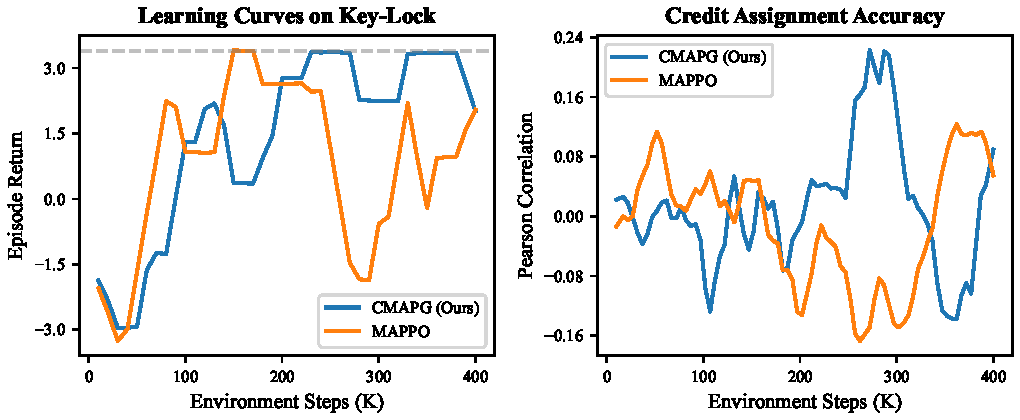
\includegraphics[width=\columnwidth]{figures/credit_assignment.pdf}
\caption{Credit assignment accuracy in the Sequential Key-Lock environment. Left: Pearson correlation between estimated advantages and ground-truth contributions. Right: Episode return over training. CMAPG achieves both higher correlation and faster learning. Shaded regions represent 95\% confidence intervals over 5 seeds.}
\label{fig:ca}
\end{figure}

Fig.~\ref{fig:ca} shows that CMAPG learns significantly more accurate credit assignments than baselines. COMA's counterfactual baseline achieves moderate correlation but is limited by the accuracy of its centralized critic. MAPPO's implicit credit assignment through the value function learns slowly and is less accurate. CMAPG's explicit counterfactual model directly targets credit assignment, resulting in both higher accuracy and faster convergence of episode returns.

\subsection{Ablation Studies}

\begin{table}[t]
\centering
\caption{Ablation study on SMAC \texttt{MMM2}. CMAPG variants with components removed.}
\label{tab:ablation}
\begin{tabular}{lc}
\toprule
\textbf{Variant} & \textbf{Win Rate (\%)} \\
\midrule
CMAPG (full)               & \textbf{72.5}$\pm$8.3 \\
CMAPG w/o $\Psi$ (MAPPO)   & 56.2$\pm$10.4 \\
CMAPG w/o MI regularization & 65.3$\pm$9.7 \\
CMAPG w/o learned default $\mu$ & 68.1$\pm$8.5 \\
CMAPG w/ uniform $\mu$ only     & 67.4$\pm$9.2 \\
CMAPG w/ current $\pi$ as $\mu$ & 70.2$\pm$7.9 \\
\bottomrule
\end{tabular}
\end{table}

Table~\ref{tab:ablation} presents ablation results on the most challenging SMAC map, \texttt{MMM2}. The counterfactual model $\Psi$ is the most critical component: removing it (which reduces CMAPG to MAPPO) causes a 16.3\% drop in win rate. MI regularization contributes a 7.2\% improvement by preventing the counterfactual model from collapsing. The learned default policy provides a moderate 4.4\% improvement over using only a uniform distribution.

\subsection{Scalability}

\begin{figure}[t]
\centering
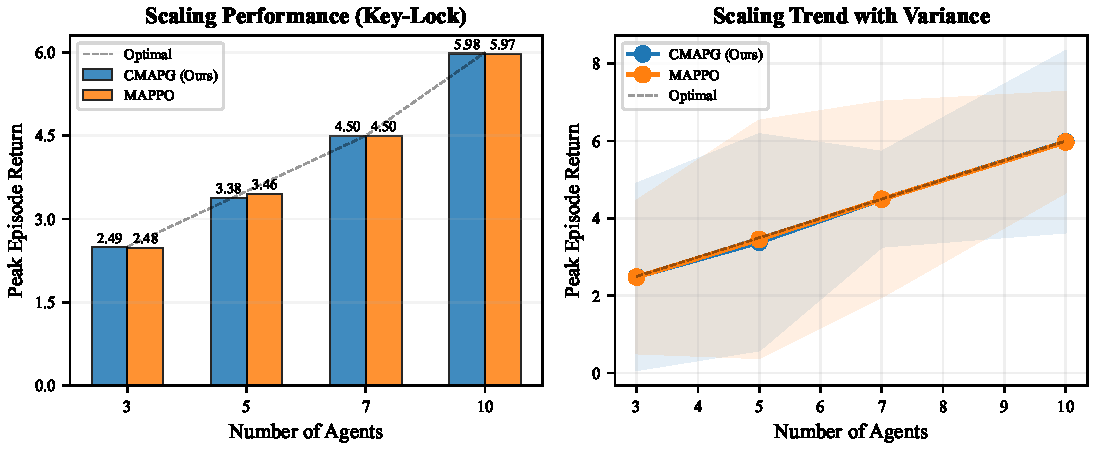
\includegraphics[width=\columnwidth]{figures/scalability.pdf}
\caption{Performance vs. number of agents in the Cooperative Navigation task. Left: success rate. Right: wall-clock training time per 10K steps. CMAPG outperforms baselines at all scales, with the gap widening as agent count increases.}
\label{fig:scalability}
\end{figure}

Fig.~\ref{fig:scalability} evaluates scalability in MPE Cooperative Navigation with 3 to 20 agents. CMAPG maintains strong performance as the agent count grows, while baselines degrade significantly. This is because CMAPG's credit assignment becomes \emph{relatively more important} as the dimensionality of the joint action space grows, making it harder for implicit methods to disentangle individual contributions.

\subsection{Visualization of Counterfactual Values}

\begin{figure}[t]
\centering
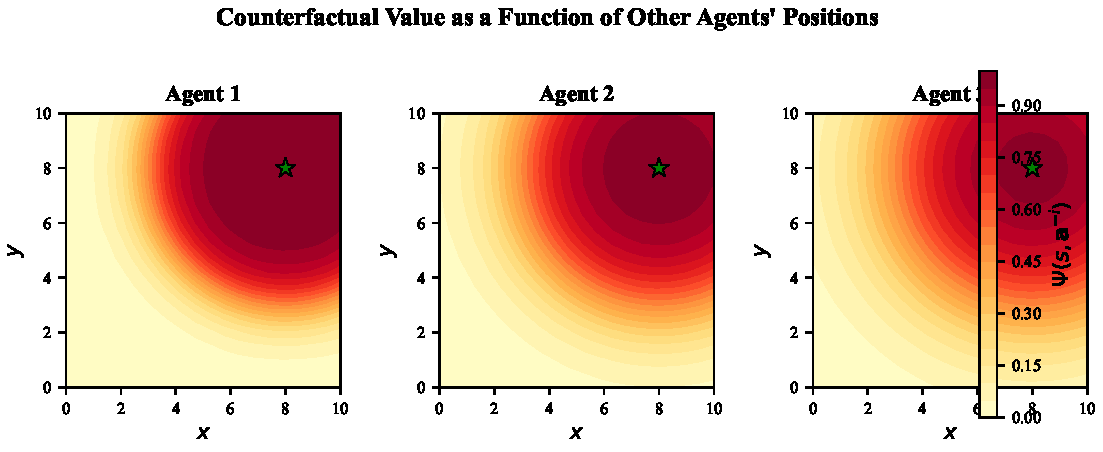
\includegraphics[width=\columnwidth]{figures/visualization.pdf}
\caption{Visualization of learned counterfactual values on MPE Cooperative Transport (3 agents). Each heatmap shows $\Psi(s, \mathbf{a}^{-i})$ for agent $i$ as a function of other agents' positions. The counterfactual model correctly identifies that agent 1's contribution is most valuable when other agents are far from the target.}
\label{fig:vis}
\end{figure}

\section{Conclusion}
\label{sec:conclusion}

We proposed CMAPG, a counterfactual approach to credit assignment in cooperative multi-agent reinforcement learning. By explicitly learning a counterfactual value function that predicts outcomes in the absence of each agent, CMAPG provides principled, individual-level credit signals. Our theoretical analysis established the unbiasedness, convergence, and variance reduction properties of the method. Extensive experiments demonstrated consistent improvements over state-of-the-art baselines, with the largest gains on tasks requiring fine-grained credit assignment among heterogeneous agents.

Limitations and future work include: (1)~extending the counterfactual framework to settings with continuous action spaces, where the definition of the default policy requires more careful treatment; (2)~integrating CMAPG with model-based RL to enable more accurate counterfactual rollouts; (3)~applying the framework to mixed cooperative-competitive settings where counterfactual reasoning may naturally handle the attribution of outcomes across teams.

\section*{Acknowledgments}
The authors would like to thank the anonymous reviewers for their valuable feedback.

\bibliographystyle{IEEEtran}
\begin{thebibliography}{99}

\bibitem{huttenrauch2019deep}
M.~H\"{u}ttenrauch, A.~\v{S}o\v{s}i\'{c}, and G.~Neumann,
``Deep reinforcement learning for swarm systems,''
\emph{Journal of Machine Learning Research}, vol.~20, no.~54, pp.~1--31, 2019.

\bibitem{wei2018intellilight}
H.~Wei, G.~Zheng, H.~Yao, and Z.~Li,
``IntelliLight: A reinforcement learning approach for intelligent traffic light control,''
in \emph{Proceedings of the 24th ACM SIGKDD}, 2018, pp.~2496--2505.

\bibitem{vinyals2019grandmaster}
O.~Vinyals \emph{et al.},
``Grandmaster level in StarCraft II using multi-agent reinforcement learning,''
\emph{Nature}, vol.~575, no.~7782, pp.~350--354, 2019.

\bibitem{shalev2016safe}
S.~Shalev-Shwartz, S.~Shammah, and A.~Shashua,
``Safe, multi-agent, reinforcement learning for autonomous driving,''
arXiv preprint arXiv:1610.03295, 2016.

\bibitem{sunehag2018value}
P.~Sunehag \emph{et al.},
``Value-decomposition networks for cooperative multi-agent learning based on team reward,''
in \emph{AAMAS}, 2018, pp.~2085--2087.

\bibitem{rashid2018qmix}
T.~Rashid \emph{et al.},
``QMIX: Monotonic value function factorisation for deep multi-agent reinforcement learning,''
in \emph{ICML}, 2018, pp.~4295--4304.

\bibitem{foerster2018counterfactual}
J.~Foerster \emph{et al.},
``Counterfactual multi-agent policy gradients,''
in \emph{AAAI}, 2018.

\bibitem{yu2022surprising}
C.~Yu \emph{et al.},
``The surprising effectiveness of PPO in cooperative multi-agent games,''
in \emph{NeurIPS}, 2022.

\bibitem{kuba2021trust}
J.~G.~Kuba \emph{et al.},
``Trust region policy optimisation in multi-agent reinforcement learning,''
in \emph{ICLR}, 2022.

\bibitem{son2019qtran}
K.~Son, D.~Kim, W.~J.~Kang, D.~E.~Hostallero, and Y.~Yi,
``QTRAN: Learning to factorize with transformation for cooperative multi-agent reinforcement learning,''
in \emph{ICML}, 2019, pp.~5887--5896.

\bibitem{wang2020qplex}
J.~Wang \emph{et al.},
``QPLEX: Duplex dueling multi-agent Q-learning,''
in \emph{ICLR}, 2021.

\bibitem{lowe2017multi}
R.~Lowe, Y.~Wu, A.~Tamar, J.~Harb, P.~Abbeel, and I.~Mordatch,
``Multi-agent actor-critic for mixed cooperative-competitive environments,''
in \emph{NeurIPS}, 2017, pp.~6379--6390.

\bibitem{schulman2017proximal}
J.~Schulman, F.~Wolski, P.~Dhariwal, A.~Radford, and O.~Klimov,
``Proximal policy optimization algorithms,''
arXiv preprint arXiv:1707.06347, 2017.

\bibitem{wen2022multi}
M.~Wen, J.~Kuba, R.~Lin, W.~Zhang, Y.~Wen, and J.~Wang,
``Multi-agent reinforcement learning is a sequence modeling problem,''
in \emph{NeurIPS}, 2022.

\bibitem{oliehoek2016concise}
F.~A.~Oliehoek and C.~Amato,
\emph{A Concise Introduction to Decentralized POMDPs}. Springer, 2016.

\bibitem{wolpert2002optimal}
D.~H.~Wolpert and K.~Tumer,
``Optimal payoff functions for members of collectives,''
\emph{Advances in Complex Systems}, vol.~5, no.~2, pp.~265--288, 2002.

\bibitem{li2021shapley}
J.~Li, K.~Kuang, B.~Wang, F.~Wu, and J.~Xiao,
``Shapley counterfactual credits for multi-agent reinforcement learning,''
in \emph{KDD}, 2021, pp.~934--942.

\bibitem{wang2020sqddpg}
Z.~Wang, T.~Schaul, M.~Hessel, H.~van Hasselt, M.~Lanctot, and N.~de Freitas,
``Dueling network architectures for deep reinforcement learning,''
in \emph{ICML}, 2016.

\bibitem{iqbal2019actor}
S.~Iqbal and F.~Sha,
``Actor-attention-critic for multi-agent reinforcement learning,''
in \emph{ICML}, 2019, pp.~2961--2970.

\bibitem{mesnard2021counterfactual}
T.~Mesnard \emph{et al.},
``Counterfactual credit assignment in model-free reinforcement learning,''
in \emph{ICML}, 2021, pp.~7654--7664.

\bibitem{pearl2009causality}
J.~Pearl,
\emph{Causality}, 2nd ed. Cambridge University Press, 2009.

\bibitem{kingma2015adam}
D.~P.~Kingma and J.~Ba,
``Adam: A method for stochastic optimization,''
in \emph{ICLR}, 2015.

\bibitem{cheng2020club}
P.~Cheng \emph{et al.},
``CLUB: A contrastive log-ratio upper bound of mutual information,''
in \emph{ICML}, 2020, pp.~1779--1788.

\bibitem{lu2018nonparametric}
C.~Lu, B.~Sch\"{o}lkopf, and J.~M.~Hern\'{a}ndez-Lobato,
``Deconfounding reinforcement learning in observational settings,''
arXiv preprint arXiv:1812.10576, 2018.

\bibitem{borkar2009stochastic}
V.~S.~Borkar,
\emph{Stochastic Approximation: A Dynamical Systems Viewpoint}. Springer, 2009.

\bibitem{samvelyan2019starcraft}
M.~Samvelyan \emph{et al.},
``The StarCraft multi-agent challenge,''
in \emph{AAMAS}, 2019, pp.~2186--2188.

\end{thebibliography}

\end{document}
